%%%% Paramétrage du cours %%%%
\def\xxactivite{Cours}
\def\xxauteur{\textsl{Xavier Pessoles \& Anthony Meurdefroid}}

\fichefalse
\proftrue
\tdfalse
\courstrue

\def\xxnumchapitre{Chapitre 2 \vspace{.2cm}}
\def\xxchapitre{\hspace{.12cm} Introduction aux réseaux de neurones}

\def\xxcompetences{%
\textsl{%
\textbf{Savoirs et compétences :}\\
\begin{itemize}[label=\ding{112},font=\color{ocre}] 
\item Analyser les principes d'intelligence artificielle.
\begin{itemize}
%\item Régression et classification, apprentissages supervisé et non supervisé.
\item Phases d'apprentissage et d'inférence.
%\item Modèle linéaire monovariable ou multivariable.
\item Réseaux de neurones (couches d'entrée, cachées et de sortie, neurones, biais, poids et fonction d'activation).
\end{itemize}
%\item Interpréter et vérifier la cohérence des résultats obtenus expérimentalement, analytiquement : Ordre de grandeur. Matrice de confusion (tableau de contingence), sensibilité et spécificité d'un test.
\item Résoudre un problème en utilisant une solution d'intelligence artificielle : 
\begin{itemize}
\item Apprentissage supervisé.
\item Choix des données d'apprentissage. 
\item Mise en œuvre des algorithmes (réseaux de neurones).
\item Phases d'apprentissage et d'inférence.
\end{itemize}
\end{itemize}
}}



\def\xxfigures{
}%figues de la page de garde

\iflivret
\pagestyle{empty}


%%%%%%%% PAGE DE GARDE COURS
\ifcours
% ==== BANDEAU DES TITRES ==== 
\begin{tikzpicture}[remember picture,overlay]
\node at (current page.north west)
{\begin{tikzpicture}[remember picture,overlay]
\node[anchor=north west,inner sep=0pt] at (0,0) {\includegraphics[width=\paperwidth]{\thechapterimage}};
\draw[anchor=west] (-2cm,-8cm) node [line width=2pt,rounded corners=15pt,draw=ocre,fill=white,fill opacity=0.6,inner sep=40pt]{\strut\makebox[22cm]{}};
\draw[anchor=west] (1cm,-8cm) node {\huge\sffamily\bfseries\color{black} %
\begin{minipage}{1cm}
\rotatebox{90}{\LARGE\sffamily\textsc{\color{ocre}\textbf{\xxnumpartie}}}
\end{minipage} \hfill
\begin{minipage}[c]{14cm}
\begin{titrepartie}
\begin{flushright}
\renewcommand{\baselinestretch}{1.1} 
\Large\sffamily\textsc{\textbf{\xxpartie}}
\renewcommand{\baselinestretch}{1} 
\end{flushright}
\end{titrepartie}
\end{minipage} \hfill
\begin{minipage}[c]{3.5cm}
{\large\sffamily\textsc{\textbf{\color{ocre} \discipline}}}
\end{minipage} 
 };
\end{tikzpicture}};
\end{tikzpicture}
% ==== FIN BANDEAU DES TITRES ==== 


% ==== ONGLET 
\begin{tikzpicture}[overlay]
\node[shape=rectangle, 
      rounded corners = .25 cm,
	  draw= ocre,
	  line width=2pt, 
	  fill = ocre!10,
	  minimum width  = 2.5cm,
	  minimum height = 3cm,] at (18.3cm,0) {};
\node at (17.7cm,0) {\rotatebox{90}{\textbf{\Large\color{ocre}{\classe}}}};
%{};
\end{tikzpicture}
% ==== FIN ONGLET 


\vspace{3.5cm}

\begin{tikzpicture}[remember picture,overlay]
\draw[anchor=west] (-2cm,-6cm) node {\huge\sffamily\bfseries\color{black} %
\begin{minipage}{2cm}
\begin{center}
\LARGE\sffamily\textsc{\color{ocre}\textbf{\xxactivite}}
\end{center}
\end{minipage} \hfill
\begin{minipage}[c]{15cm}
\begin{titrechapitre}
\renewcommand{\baselinestretch}{1.1} 
\Large\sffamily\textsc{\textbf{\xxnumchapitre}}

\Large\sffamily\textsc{\textbf{\xxchapitre}}
\vspace{.5cm}

\renewcommand{\baselinestretch}{1} 
\normalsize\normalfont
\xxcompetences
\end{titrechapitre}
\end{minipage}  };
\end{tikzpicture}
\vfill

\begin{flushright}
\begin{minipage}[c]{.3\linewidth}
\begin{center}
\xxfigures
\end{center}
\end{minipage}\hfill
\begin{minipage}[c]{.6\linewidth}
\startcontents
%\printcontents{}{1}{}
\printcontents{}{1}{}
\end{minipage}
\end{flushright}

\begin{tikzpicture}[remember picture,overlay]
\draw[anchor=west] (4.5cm,-.7cm) node {
\begin{minipage}[c]{.2\linewidth}
\begin{flushright}

\includegraphics[width=2cm]{logoCC}
\end{flushright}
\end{minipage}
\begin{minipage}[c]{.2\linewidth}
\textsl{\xxauteur} \\
\textsl{\classe}
\end{minipage}
 };
\end{tikzpicture}

\newpage
\pagestyle{fancy}

%\newpage
%\pagestyle{fancy}

\else
\fi
%% FIN PAGE DE GARDE DES COURS

%%%%%%%% PAGE DE GARDE TD
\iftd

% BANDEAU EXO
\iflivret % SI LIVRET ET TD
\begin{tikzpicture}[remember picture,overlay]
\draw[anchor=west] (-2cm,-3.3cm) node {\huge\sffamily\bfseries\color{black} %
\begin{minipage}{5cm}
\begin{center}
\LARGE\sffamily\color{ocre}\textbf{\textsc{\xxactivite}}

\begin{center}
\xxfigures
\end{center}

\end{center}
\end{minipage} \hfill
\begin{minipage}[c]{12cm}
\begin{titrechapitre}
\renewcommand{\baselinestretch}{1.1} 
\large\sffamily\textbf{\textsc{\xxtitreexo}}

\small\sffamily{\textbf{\textit{\color{black!70}\xxsourceexo}}}
\vspace{.5cm}

\renewcommand{\baselinestretch}{1} 
\normalsize\normalfont
\xxcompetences
\end{titrechapitre}
\end{minipage}};
\end{tikzpicture}
\else % ELSE NOT LIVRET
\begin{tikzpicture}[remember picture,overlay]
\draw[anchor=west] (-2cm,-3.5cm) node {\huge\sffamily\bfseries\color{black} %
\begin{minipage}{5cm}
\begin{center}
\LARGE\sffamily\color{ocre}\textbf{\textsc{\xxactivite}}

\begin{center}
\xxfigures
\end{center}

\end{center}
\end{minipage} \hfill
\begin{minipage}[c]{12cm}
\begin{titrechapitre}
\renewcommand{\baselinestretch}{1.1} 
\large\sffamily\textbf{\textsc{\xxtitreexo}}

\small\sffamily{\textbf{\textit{\color{black!70}\xxsourceexo}}}
\vspace{.5cm}

\renewcommand{\baselinestretch}{1} 
\normalsize\normalfont
\xxcompetences
\end{titrechapitre}
\end{minipage}};
\end{tikzpicture}

\fi

\else   % FIN IF TD
\fi


%%%%%%%% PAGE DE GARDE FICHE
\iffiche
\begin{tikzpicture}[remember picture,overlay]
\node at (current page.north west)
{\begin{tikzpicture}[remember picture,overlay]
\draw[anchor=west] (-2cm,\xxYCartouche) node [line width=2pt,rounded corners=15pt,draw=ocre,fill=white,fill opacity=0.6,inner sep=40pt]{\strut\makebox[22cm]{}};
\draw[anchor=west] (1cm,\xxYCartouche) node {\huge\sffamily\bfseries\color{black} %
\begin{minipage}{1cm}
\rotatebox{90}{\LARGE\sffamily\textsc{\color{ocre}\textbf{\xxnumpartie}}}
\end{minipage} \hfill
\begin{minipage}[c]{14cm}
\begin{titrepartie}
\begin{flushright}
\renewcommand{\baselinestretch}{1.1} 
\large\sffamily\textsc{\textbf{\xxpartie} \\} 

\vspace{.2cm}

\normalsize\sffamily\textsc{\textbf{\xxnumchapitre -- \xxchapitre}}
\renewcommand{\baselinestretch}{1} 
\end{flushright}
\end{titrepartie}
\end{minipage} \hfill
\begin{minipage}[c]{3.5cm}
{\large\sffamily\textsc{\textbf{\color{ocre} \discipline}}}
\end{minipage} 
 };
\end{tikzpicture}};
\end{tikzpicture}

\iflivret % SI LIVRET
\begin{tikzpicture}[overlay]
\node[shape=rectangle, 
      rounded corners = .25 cm,
	  draw= ocre,
	  line width=2pt, 
	  fill = ocre!10,
	  minimum width  = 2.5cm,
	  minimum height = 2.5cm,] at (18.5cm,\xxYongletGarde) {};
\node at (17.9cm,\xxYongletGarde) {\rotatebox{90}{\textsf{\textbf{\large\color{ocre}{\classe}}}}};
%{};
\end{tikzpicture}
\else  % SI PAS LIVRET
\iftd %% SI TD et PAS LIVRET
\begin{tikzpicture}[overlay]
\node[shape=rectangle, 
      rounded corners = .25 cm,
	  draw= ocre,
	  line width=2pt, 
	  fill = ocre!10,
	  minimum width  = 2.5cm,
	  minimum height = 2.5cm,] at (18.6cm,\xxYOnget) {}; %% 0.9 par défaut
\node at (18cm,\xxYOnget) {\rotatebox{90}{\textsf{\textbf{\large\color{ocre}{\classe}}}}};
%{};
\end{tikzpicture}

\else % FIN DU SI TD PAS LIVRET 
\begin{tikzpicture}[overlay]
\node[shape=rectangle, 
      rounded corners = .25 cm,
	  draw= ocre,
	  line width=2pt, 
	  fill = ocre!10,
	  minimum width  = 2.5cm,
%	  minimum height = 2.5cm,] at (18.5cm,1.1cm) {}; % \xxYOnget 0.5
	  minimum height = 2.5cm,] at (18.6cm,.5cm) {};
\node at (18cm,.5cm) {\rotatebox{90}{\textsf{\textbf{\large\color{ocre}{\classe}}}}};
%{};
\end{tikzpicture}
\fi
\fi
\else
\fi



\else
\pagestyle{empty}


%%%%%%%% PAGE DE GARDE COURS
\ifcours
% ==== BANDEAU DES TITRES ==== 
\begin{tikzpicture}[remember picture,overlay]
\node at (current page.north west)
{\begin{tikzpicture}[remember picture,overlay]
\node[anchor=north west,inner sep=0pt] at (0,0) {\includegraphics[width=\paperwidth]{\thechapterimage}};
\draw[anchor=west] (-2cm,-8cm) node [line width=2pt,rounded corners=15pt,draw=ocre,fill=white,fill opacity=0.6,inner sep=40pt]{\strut\makebox[22cm]{}};
\draw[anchor=west] (1cm,-8cm) node {\huge\sffamily\bfseries\color{black} %
\begin{minipage}{1cm}
\rotatebox{90}{\LARGE\sffamily\textsc{\color{ocre}\textbf{\xxnumpartie}}}
\end{minipage} \hfill
\begin{minipage}[c]{14cm}
\begin{titrepartie}
\begin{flushright}
\renewcommand{\baselinestretch}{1.1} 
\Large\sffamily\textsc{\textbf{\xxpartie}}
\renewcommand{\baselinestretch}{1} 
\end{flushright}
\end{titrepartie}
\end{minipage} \hfill
\begin{minipage}[c]{3.5cm}
{\large\sffamily\textsc{\textbf{\color{ocre} \discipline}}}
\end{minipage} 
 };
\end{tikzpicture}};
\end{tikzpicture}
% ==== FIN BANDEAU DES TITRES ==== 


% ==== ONGLET 
\begin{tikzpicture}[overlay]
\node[shape=rectangle, 
      rounded corners = .25 cm,
	  draw= ocre,
	  line width=2pt, 
	  fill = ocre!10,
	  minimum width  = 2.5cm,
	  minimum height = 3cm,] at (18.3cm,0) {};
\node at (17.7cm,0) {\rotatebox{90}{\textbf{\Large\color{ocre}{\classe}}}};
%{};
\end{tikzpicture}
% ==== FIN ONGLET 


\vspace{3.5cm}

\begin{tikzpicture}[remember picture,overlay]
\draw[anchor=west] (-2cm,-6cm) node {\huge\sffamily\bfseries\color{black} %
\begin{minipage}{2cm}
\begin{center}
\LARGE\sffamily\textsc{\color{ocre}\textbf{\xxactivite}}
\end{center}
\end{minipage} \hfill
\begin{minipage}[c]{15cm}
\begin{titrechapitre}
\renewcommand{\baselinestretch}{1.1} 
\Large\sffamily\textsc{\textbf{\xxnumchapitre}}

\Large\sffamily\textsc{\textbf{\xxchapitre}}
\vspace{.5cm}

\renewcommand{\baselinestretch}{1} 
\normalsize\normalfont
\xxcompetences
\end{titrechapitre}
\end{minipage}  };
\end{tikzpicture}
\vfill

\begin{flushright}
\begin{minipage}[c]{.3\linewidth}
\begin{center}
\xxfigures
\end{center}
\end{minipage}\hfill
\begin{minipage}[c]{.6\linewidth}
\startcontents
%\printcontents{}{1}{}
\printcontents{}{1}{}
\end{minipage}
\end{flushright}

\begin{tikzpicture}[remember picture,overlay]
\draw[anchor=west] (4.5cm,-.7cm) node {
\begin{minipage}[c]{.2\linewidth}
\begin{flushright}

\includegraphics[width=2cm]{logoCC}
\end{flushright}
\end{minipage}
\begin{minipage}[c]{.2\linewidth}
\textsl{\xxauteur} \\
\textsl{\classe}
\end{minipage}
 };
\end{tikzpicture}

\newpage
\pagestyle{fancy}

%\newpage
%\pagestyle{fancy}

\else
\fi
%% FIN PAGE DE GARDE DES COURS

%%%%%%%% PAGE DE GARDE TD
\iftd

% BANDEAU EXO
\iflivret % SI LIVRET ET TD
\begin{tikzpicture}[remember picture,overlay]
\draw[anchor=west] (-2cm,-3.3cm) node {\huge\sffamily\bfseries\color{black} %
\begin{minipage}{5cm}
\begin{center}
\LARGE\sffamily\color{ocre}\textbf{\textsc{\xxactivite}}

\begin{center}
\xxfigures
\end{center}

\end{center}
\end{minipage} \hfill
\begin{minipage}[c]{12cm}
\begin{titrechapitre}
\renewcommand{\baselinestretch}{1.1} 
\large\sffamily\textbf{\textsc{\xxtitreexo}}

\small\sffamily{\textbf{\textit{\color{black!70}\xxsourceexo}}}
\vspace{.5cm}

\renewcommand{\baselinestretch}{1} 
\normalsize\normalfont
\xxcompetences
\end{titrechapitre}
\end{minipage}};
\end{tikzpicture}
\else % ELSE NOT LIVRET
\begin{tikzpicture}[remember picture,overlay]
\draw[anchor=west] (-2cm,-3.5cm) node {\huge\sffamily\bfseries\color{black} %
\begin{minipage}{5cm}
\begin{center}
\LARGE\sffamily\color{ocre}\textbf{\textsc{\xxactivite}}

\begin{center}
\xxfigures
\end{center}

\end{center}
\end{minipage} \hfill
\begin{minipage}[c]{12cm}
\begin{titrechapitre}
\renewcommand{\baselinestretch}{1.1} 
\large\sffamily\textbf{\textsc{\xxtitreexo}}

\small\sffamily{\textbf{\textit{\color{black!70}\xxsourceexo}}}
\vspace{.5cm}

\renewcommand{\baselinestretch}{1} 
\normalsize\normalfont
\xxcompetences
\end{titrechapitre}
\end{minipage}};
\end{tikzpicture}

\fi

\else   % FIN IF TD
\fi


%%%%%%%% PAGE DE GARDE FICHE
\iffiche
\begin{tikzpicture}[remember picture,overlay]
\node at (current page.north west)
{\begin{tikzpicture}[remember picture,overlay]
\draw[anchor=west] (-2cm,\xxYCartouche) node [line width=2pt,rounded corners=15pt,draw=ocre,fill=white,fill opacity=0.6,inner sep=40pt]{\strut\makebox[22cm]{}};
\draw[anchor=west] (1cm,\xxYCartouche) node {\huge\sffamily\bfseries\color{black} %
\begin{minipage}{1cm}
\rotatebox{90}{\LARGE\sffamily\textsc{\color{ocre}\textbf{\xxnumpartie}}}
\end{minipage} \hfill
\begin{minipage}[c]{14cm}
\begin{titrepartie}
\begin{flushright}
\renewcommand{\baselinestretch}{1.1} 
\large\sffamily\textsc{\textbf{\xxpartie} \\} 

\vspace{.2cm}

\normalsize\sffamily\textsc{\textbf{\xxnumchapitre -- \xxchapitre}}
\renewcommand{\baselinestretch}{1} 
\end{flushright}
\end{titrepartie}
\end{minipage} \hfill
\begin{minipage}[c]{3.5cm}
{\large\sffamily\textsc{\textbf{\color{ocre} \discipline}}}
\end{minipage} 
 };
\end{tikzpicture}};
\end{tikzpicture}

\iflivret % SI LIVRET
\begin{tikzpicture}[overlay]
\node[shape=rectangle, 
      rounded corners = .25 cm,
	  draw= ocre,
	  line width=2pt, 
	  fill = ocre!10,
	  minimum width  = 2.5cm,
	  minimum height = 2.5cm,] at (18.5cm,\xxYongletGarde) {};
\node at (17.9cm,\xxYongletGarde) {\rotatebox{90}{\textsf{\textbf{\large\color{ocre}{\classe}}}}};
%{};
\end{tikzpicture}
\else  % SI PAS LIVRET
\iftd %% SI TD et PAS LIVRET
\begin{tikzpicture}[overlay]
\node[shape=rectangle, 
      rounded corners = .25 cm,
	  draw= ocre,
	  line width=2pt, 
	  fill = ocre!10,
	  minimum width  = 2.5cm,
	  minimum height = 2.5cm,] at (18.6cm,\xxYOnget) {}; %% 0.9 par défaut
\node at (18cm,\xxYOnget) {\rotatebox{90}{\textsf{\textbf{\large\color{ocre}{\classe}}}}};
%{};
\end{tikzpicture}

\else % FIN DU SI TD PAS LIVRET 
\begin{tikzpicture}[overlay]
\node[shape=rectangle, 
      rounded corners = .25 cm,
	  draw= ocre,
	  line width=2pt, 
	  fill = ocre!10,
	  minimum width  = 2.5cm,
%	  minimum height = 2.5cm,] at (18.5cm,1.1cm) {}; % \xxYOnget 0.5
	  minimum height = 2.5cm,] at (18.6cm,.5cm) {};
\node at (18cm,.5cm) {\rotatebox{90}{\textsf{\textbf{\large\color{ocre}{\classe}}}}};
%{};
\end{tikzpicture}
\fi
\fi
\else
\fi



\fi
\setlength{\columnseprule}{.1pt}

\vspace{2cm}
\pagestyle{fancy}
\thispagestyle{plain}

\section{Introduction}

\subsection{Bref historique}

\subsection{Exemples d'applications des réseaux de neurones}

\section{Le neurone, les réseaux de neurones}

\subsection{Modèle de neurone}

\begin{defi}[Neurone (ou perceptron)] ~\\


\begin{minipage}[c]{.55\linewidth}
Prenons la représentation suivante pour un neurone. On note :
\begin{itemize}
\item $\mathbf{X}$ le vecteur d'entrée et $x_i$ les données de la couche d'entrée;
\item $w_i$ les poids (poids synaptiques);
\item $b$ le biais;
\item $z_0$ la somme pondérée des entrée;
\item $f$ une fonction d'activation; 
\item $\tilde{y}_0$ : la valeur de sortie du neurone.
\end{itemize}
\end{minipage}
\hfill
\begin{minipage}[c]{.4\linewidth}
\begin{center}
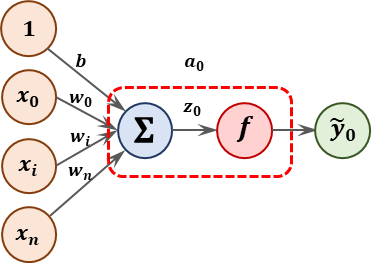
\includegraphics[width=.9\linewidth]{images/fig_01}
\end{center}
\end{minipage}

On a donc, dans un premier temps  :
$$z_0 = b+ \sum\limits_{i=0}^{n} w_i x_i. $$

Après la fonction d'activation, on a donc en sortie du neurone :
$$\tilde{y}_0 = f(z_0)=f \left( b+ \sum\limits_{i=0}^{n} w_i x_i\right).$$

\begin{rem}
\begin{enumerate}
\item La notation tilde ($\tilde{y}_0$) vient du fait que la valeur de sortie d'une neurone est une valeur estimée qu'il faudra comparer à ${y}_0$ valeur de l'étiquette utilisée pour l'apprentissage supervisé.
\item Par la suite, dans la représentation graphique on ne fera pas apparaître la somme pondérée et la fonction d'activation, mais seulement la valeur de sortie du neurone (notée par exemple $a_0$).
\end{enumerate}
\end{rem}

\end{defi}




\begin{defi}[Fonction d'activation]

Les fonctions d'activation sont des fonctions mathématiques appliquées au signal de sortie ($z$). Il est alors possible d'ajouter des non linéarités à la somme pondérée. On donne ci-dessous quelques fonctions usuelles : 

\begin{center}
\begin{tabular}{|c|c|c|c|}
\hline 
Identité & Heaviside & Logistique & Unité de rectification \\
  &  & (sigmoïde) &  linéaire (ReLU) \\
\hline 
&&&\\
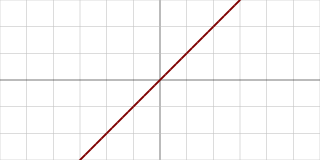
\includegraphics[width=2cm]{images/fig_03_Identite} &
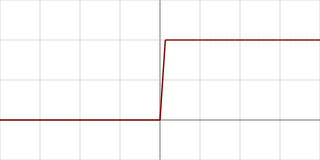
\includegraphics[width=2cm]{images/fig_03_heaviside} &
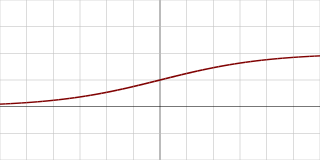
\includegraphics[width=2cm]{images/fig_03_Logistique} &
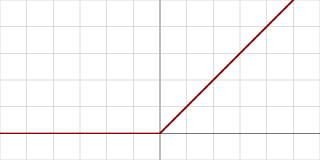
\includegraphics[width=2cm]{images/fig_03_ReLU} \\
&&&\\
$f(x)=x$ & 
$f(x)=\left\{
\begin{array}{l} 
0 \text{ si } x<0 \\ 1 \text{ si } x \geq 0 \\
 \end{array}\right. $
&
$ f(x) = \dfrac{1}{1+\text{e}^{-x}}$ &
$f(x)=\left\{
\begin{array}{l} 
0 \text{ si } x<0 \\ x \text{ si } x \geq 0 \\
 \end{array}\right. $ \\
\hline 
\end{tabular}
\end{center}

\end{defi}


\begin{rem}
Influence des poids et des biais sur la sortie du perceptron en utilisant une fonction d'activation ReLU.

\begin{minipage}[c]{.45\linewidth}
\begin{center}
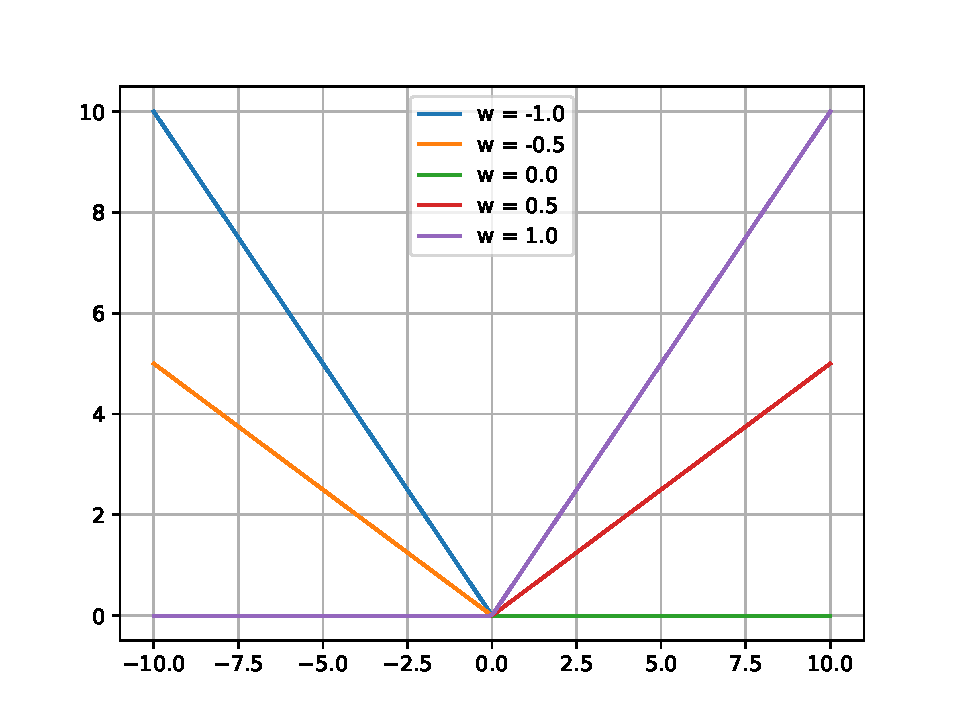
\includegraphics[width=.9\linewidth]{images/poids}
\end{center}
\end{minipage}
\hfill
\begin{minipage}[c]{.45\linewidth}
\begin{center}
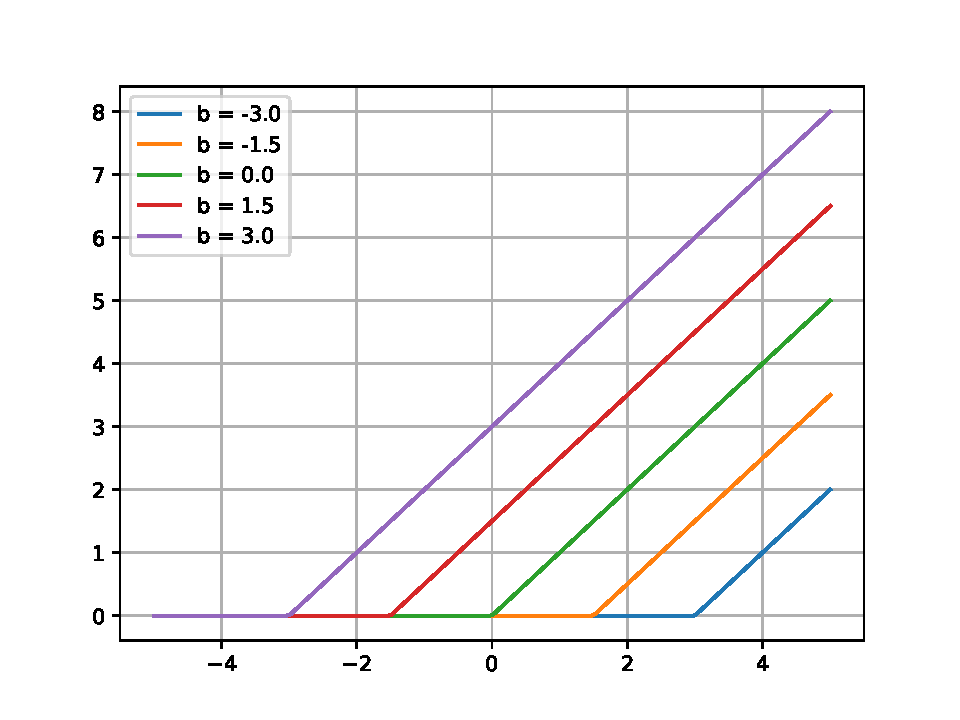
\includegraphics[width=.9\linewidth]{images/biais}
\end{center}
\end{minipage}

On peut ainsi voir qu'avec la fonction d'activation ReLU, plus le poids sera grand en valeur absolu, plus la neurone amplifiera le signal d'entrée. 

Le biais permettra de prendre en compte le << niveau >> du signal d'entrée à partir duquel, le signal doit être amplifié, ou non.

\end{rem}


\begin{exemple}~\\



\begin{minipage}[c]{.4\linewidth}

Prenons un neurone à deux entrées binaires. 
Initialisation les poids et le biais avec des valeurs aléatoires : $w_0 = -0,3$, $w_1 = 0,8$ et $b=0,2$.

\begin{center}
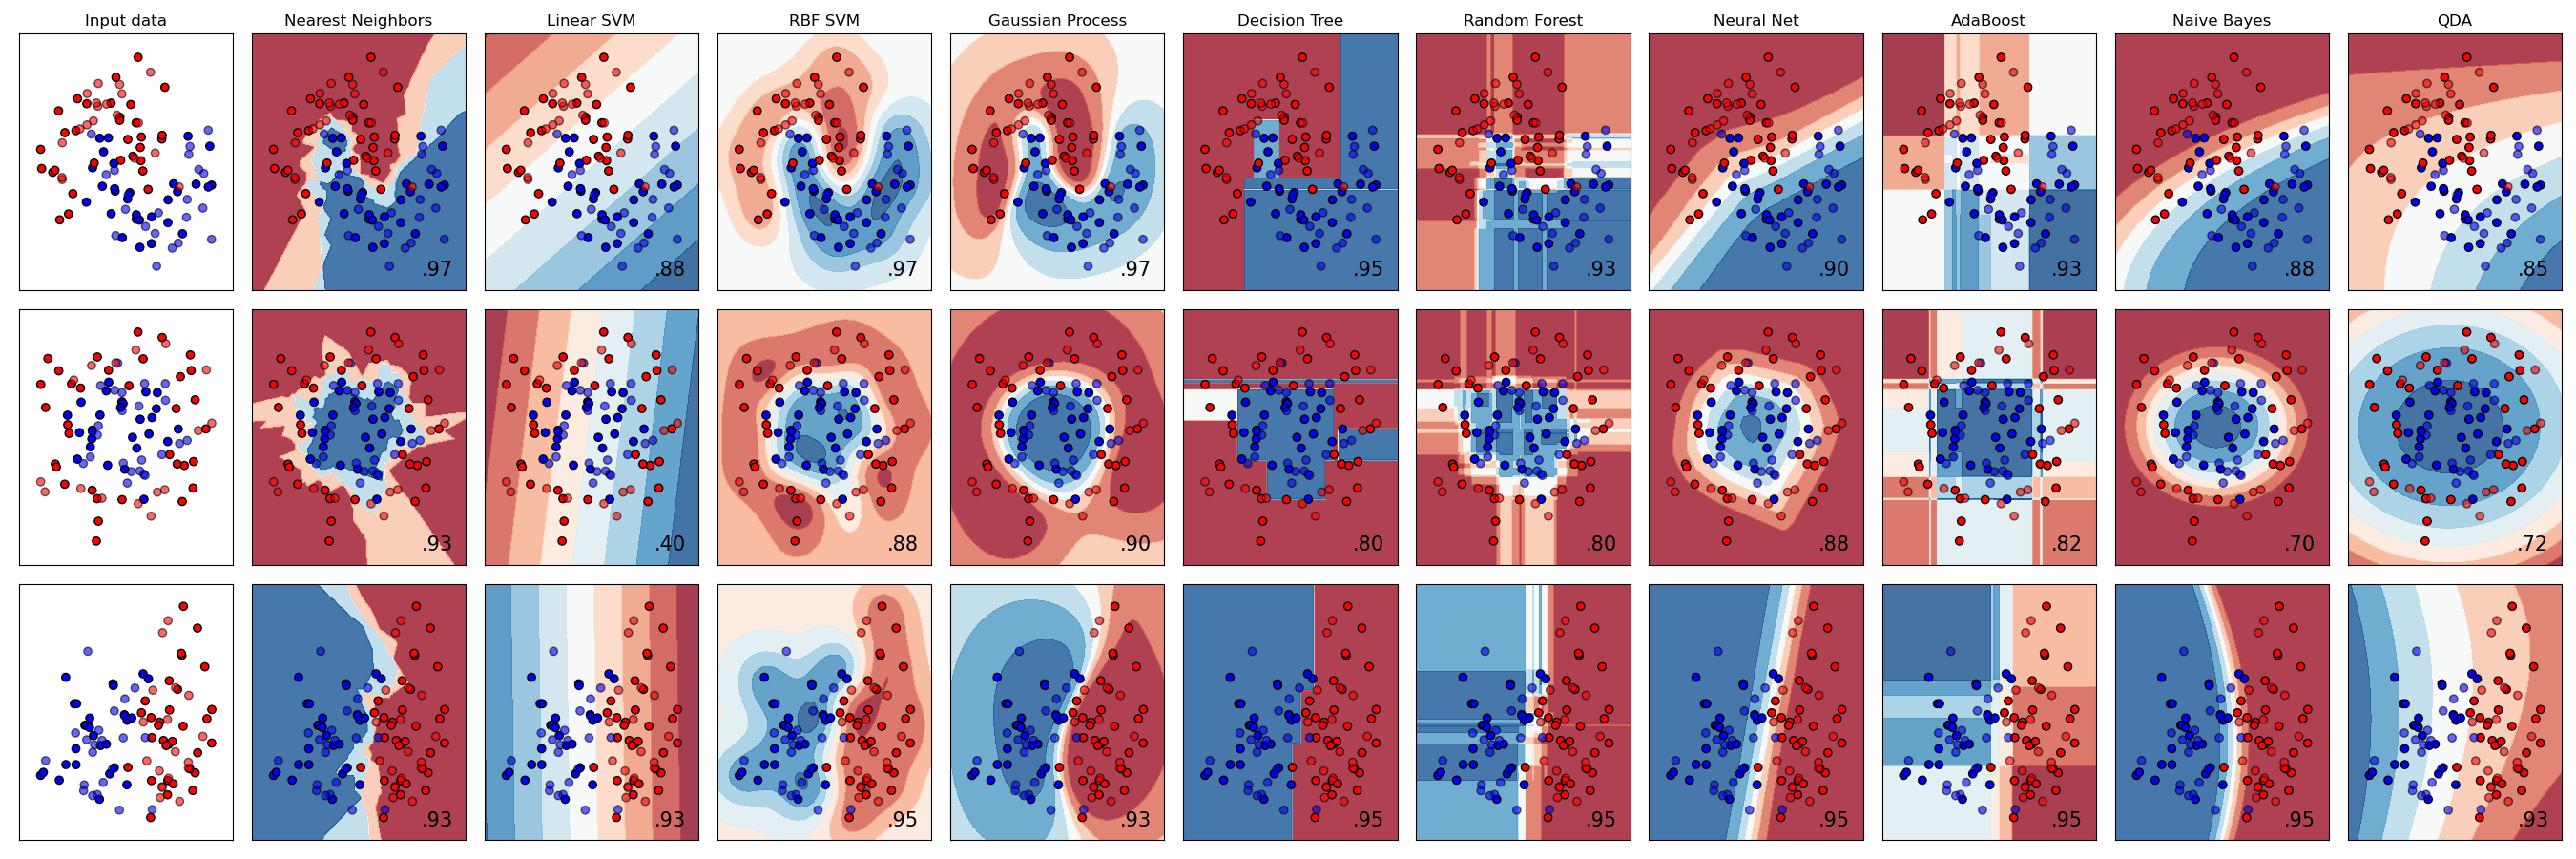
\includegraphics[width=.9\linewidth]{images/fig_02}
\end{center}
\hfill
\end{minipage}
\begin{minipage}[c]{.55\linewidth}


On peut donc évaluer l'ensemble des sorties calculable par le neurone.

\begin{center}
\begin{tabular}{|c|c|| c || c| c|c|c|}
\hline
$x_0$ & $x_1$ & $z$ & Id. & H. & Sig. & ReLu \\
\hline
\hline
0 & 0 & 0,2   &   0,2   &  1 & 0.549 & 0,2 \\
0 & 1 & 1     &    1     &  1 & 0.731  & 1\\
1 & 0 & -0.1  &    -0.1 &  0 &0.475 & 0 \\
1 & 1 & 0.7  &     0.7  &  1 &0.668 & 0.7\\
\hline
\end{tabular}
\end{center}
\end{minipage}

\end{exemple}


\section{Réseaux de neurones}
\url{https://playground.tensorflow.org/}
%LSTM


\subsection{Modélisation d'un réseau de neurones} 

\begin{defi}[Couches] ~\\

Un réseau de neurones est un ensemble de neurones reliés, par couches, entre eux. 

Dans un réseau de neurones \textbf{dense} tous les neurones de la couche $i$ seront reliés à tous les neurones de la couche $i+1$.

\begin{itemize}
\item Couche d'entrée : cette couche est une copie de l'ensemble des données d'entrées. Le nombre de neurones de cette couche correspond donc aux nombre de données d'entrées. On note $\mathbf{X} = \left( x_0, ..., x_n\right)$ le vecteur d'entrées.
\item Couche cachée (ou couche intermédiaire) : il s'agit d'une couche qui a une utilité intrinsèque au réseau de neurones. Ajouter des neurone dans cette couche (ou ces couches) permet donc d'ajouter de nouveaux paramètres.  Pour une couche, la même fonction d'activation est utilisée pour tous les neurones. En revanche la fonction d'activation utilisée peut être différente pour deux couches différentes. Les fonctions d'activations des couches intermédiaires sont souvent non linéaires.
\item Couche de sortie : le nombre de neurones de cette couche correspond au nombre de sorties attendues. La fonction d'activation de la couche de sortie est souvent linéaire. On note $\mathbf{Y} = \left( y_0, ..., y_y\right)$ le vecteur des sorties.
\end{itemize}
%\begin{minipage}[c]{.5\linewidth}
\begin{center}

\includegraphics[width=.8\linewidth]{images/fig_04}
\end{center}
%\end{minipage}

En utilisant la loi de comportement du modèle de perceptron, on peut donc exprimer $\mathbf{Y}=\mathcal{F}\left(\mathbf{X}\right)$ 
où $\mathcal{F}$ est une fonction dépendant des entrées, des poids et des biais.


Notations : 
\begin{itemize}
\item on note $w^{[\ell]}_{jk}$ les poids permettant d'aller vers la couche $\ell$ depuis le neurone $k$ vers le neurone $j$;
\item $b^{[\ell]}_{j}$ le biais permettant d'aller sur le neurone $j$ de la couche $\ell$;
\item $f^{[\ell]}$ la fonction d'activation de la couche $\ell$;
\item $n^{[\ell]}$ le nombre de neurones de la couche $\ell$.
\end{itemize}
\end{defi}

\begin{defi}[Équation de propagation]

Pour chacun des neurones $a_j^{[\ell]}$ on peut donc écrire l'équation de propagation qui lui est associé : 
$$
a_j^{[\ell]} = f^{[\ell]}\left(\sum\limits_{k=0}^{n^{[\ell-1]}}\left( w^{[\ell]}_{jk} a_k^{[\ell-1]} \right) + b^{[\ell]}_{j}\right) = f^{[\ell]}\left(z_j^{[\ell]}\right).
$$

\end{defi}


\begin{exemple}~\\

\begin{minipage}[c]{.4\linewidth}

Prenons un réseau de neurones à 3 couches : 
\begin{itemize}
\item 1 couche d'entrée à 2 neurones;
\item 1 couche cachée à 2 neurones, de fonction d'activation $f_1$;
\item 1 couche de sortie à 1 neurone, de fonction d'activation $f_2$; 
\end{itemize}

Initialisation les poids et le biais avec des valeurs aléatoires : $w_0 = -0,3$, $w_1 = 0,8$ et $b=0,2$.



\end{minipage}\hfill
\begin{minipage}[c]{.55\linewidth}
\begin{center}
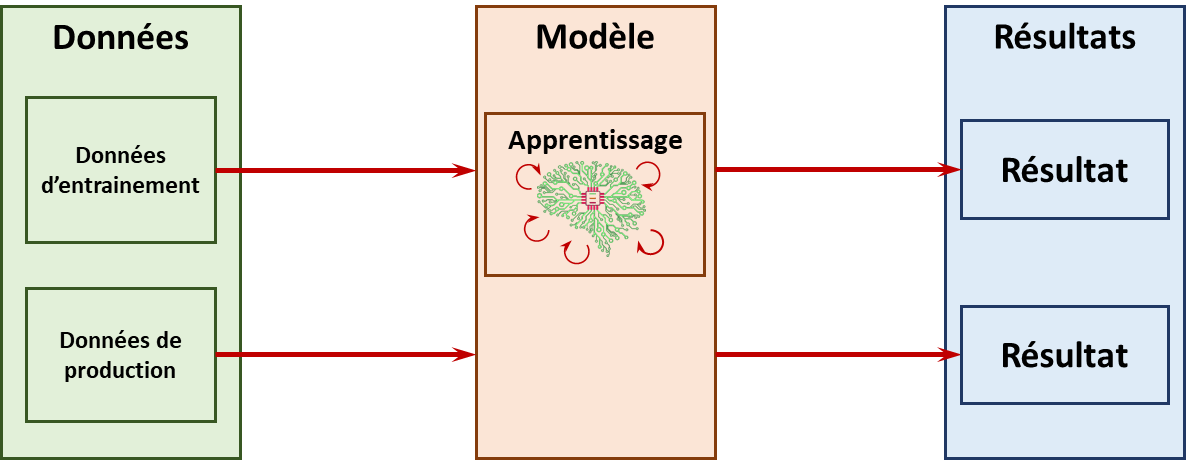
\includegraphics[width=.9\linewidth]{images/fig_05}
\end{center}
%On peut donc évaluer l'ensemble des sorties calculable par le neurone.
%
%\begin{center}
%\begin{tabular}{|c|c|| c || c| c|c|c|}
%\hline
%$x_0$ & $x_1$ & $z$ & Id. & H. & Sig. & ReLu \\
%\hline
%\hline
%0 & 0 & 0,2   &   0,2   &  1 & 0.549 & 0,2 \\
%0 & 1 & 1     &    1     &  1 & 0.731  & 1\\
%1 & 0 & -0.1  &    -0.1 &  0 &0.475 & 0 \\
%1 & 1 & 0.7  &     0.7  &  1 &0.668 & 0.7\\
%\hline
%\end{tabular}
%\end{center}
\end{minipage}

Il est possible d'écrire que 
$y_0 = a_0^{[1]}$ 
$ = f_2\left(b_0^{[2]}+ w_{00}^{[2]} a_0^{[1]}+ w_{01}^{[2]} a_1^{[1]}\right)$.

Par ailleurs : 
 $  a_0^{[1]}$ 
$ = f_1\left(b_0^{[1]}+ w_{00}^{[1]} a_0^{[0]}+ w_{01}^{[1]} a_1^{[0]}\right)$ et
  $  a_1^{[1]}$ 
$ = f_1\left(b_1^{[1]}+ w_{10}^{[1]} a_0^{[0]}+ w_{11}^{[1]} a_1^{[0]}\right)$.

Au final, on a donc 

$y_0 = a_0^{[1]}$
$ =  f_2\left(b_0^{[2]}+ w_{00}^{[2]}\left(f_1\left(b_0^{[1]}+ w_{00}^{[1]} a_0^{[0]}+ w_{01}^{[1]} a_1^{[0]}\right)\right)+ w_{01}^{[2]} \left( f_1\left(b_1^{[1]}+ w_{10}^{[1]} a_0^{[0]}+ w_{11}^{[1]} a_1^{[0]}\right)\right)\right) $ 


\end{exemple}

\begin{defi}[Paramètres]

Les paramètres du réseau de neurones sont les poids et les biais, autant de valeurs que l’entraînement devra déterminer.

\end{defi}
\begin{methode}[Calcul du nombre de paramètres -- à vérifier] ~\\

Soit un jeu de données étiquetées avec $n$ entrées et $p$ sorties.

On construit un réseau possédant $\ell$ couches  et $a_\ell$ le nombre de neurones de la couche  $\ell$. Dans ce cas, la première couche est la couche d'entrée ($a_1 = n$) et la dernière couche et la couche de sortie ($a_\ell= p$).


\textbf{Nombre de poids :} $n_w = \sum\limits_{i=1}^{\ell-1} \left(a_i \times a_{i+1}\right)$.

\textbf{Nombre de bais :} $n_b = \sum\limits_{i=2}^{\ell}\left( a_i  \right)$.


Au final, le nombre total de paramètre à calculer est donné par $N=n_w+n_b$.

\end{methode}
\begin{obj}
Soit un jeu de données étiquetées. On note $\mathbf{X}$ le vecteur des données d'entrées. On note $\mathbf{Y}$ le vecteur des données de sorties. On note
$\mathbf{\tilde{Y}}$ le vecteur de sortie calculé par le réseau de neurones.


L'objectif de la phase d'apprentissage du réseau de neurones est de déterminer les valeurs de  l'ensemble des poids et des biais de telle sorte que l'écart entre $\mathbf{Y}$ 
et $\mathbf{\tilde{Y}}$ soit minimale.
\end{obj}




\subsection{Fonction de coût}
Dans le but de minimiser l'écart entre la sortie du réseau de neurones et la valeur réelle de la sortie, on utilise une fonction côut (ou fonction de perte). Il est possible de définir plusieurs types de fonctions, notamment en fonction du type de problème à traiter (classification ou régression par exemple).

\begin{defi}[Fonction coût régression]
Notons $nb$ le nombre de données dans la base d'entraînement. Dans le cadre d'un problème de régression, on peut définir la fonction coût comme la moyenne des erreurs quadratique entre la valeur donnée par l'équation de propagation et la valeur de l'étiquette :
$$
C = \dfrac{1}{nb} \sum \limits_{i=1}^{nb} \left( \mathbf{\tilde{Y_i}} - \mathbf{Y_i}  \right)^2
$$
\end{defi}
\begin{obj}
L'objectif est dès lors de minimiser cette fonction.
\end{obj}



\subsection{Notion de rétropropagation}


\begin{defi}[Quantification de l'erreur]
\end{defi}


\subsection{Suraprentissage}

\section{Pour aller plus loin...}

Analyse d'image et réseaux convolutifs. 
Times series...

Exemples : 
\url{https://makina-corpus.com/blog/metier/2017/initiation-au-machine-learning-avec-python-pratique}

\begin{thebibliography}{2}
   \bibitem[1]{ref1} Éric Biernat et Michel Lutz. {\it Data science : fondamentaux et études de cas.} Eyrolles.
\end{thebibliography}

